\documentclass[10pt,aspectratio=169]{beamer}

\usepackage[T1]{fontenc}
\usepackage{lmodern}

\usepackage{amsmath,amssymb,mathtools}
\usepackage{bm}
\usepackage{empheq}
\usepackage{graphicx}
\usepackage{array,booktabs,tabularx,tabulary,multirow}
\usepackage{tikz}
\usepackage{hyperref}
\usepackage{feynmp}

\newcolumntype{V}{>{\centering\arraybackslash} m{.2\linewidth} }

\usetikzlibrary{arrows,matrix,shapes,positioning}
\usetikzlibrary{calc}

\newcommand*\widefbox[1]{\fbox{\hspace{0.5em}#1\hspace{0.5em}}}
\newcommand{\DRbar}{{\overline{\textrm{DR}}}}

\DeclareGraphicsRule{*}{mps}{*}{}
\graphicspath{{./figures/}}

\title{Naturalness, Dark Matter and $E_6$ Inspired SUSY Models}

\author{D.~Harries\\
  {\scriptsize
  (IPNP, Charles University in Prague)}\\
  \vspace{25pt}
  { \scriptsize
    Based on:\\[3mm]
  }
  { \tiny
    \href{https://doi.org/10.1103/PhysRevD.91.115024}{%
      P.~Athron, D.~Harries, and A.~G.~Williams, Phys.~Rev.~\textbf{D91},
      115024}
         [\href{https://arxiv.org/abs/1503.08929}{arXiv:1503.08929}]\\[2mm]
    \href{https://doi.org/10.1016/j.physletb.2016.06.040}{%
      P.~Athron, D.~Harries, R.~Nevzorov, and A.~G.~Williams,
      Phys.~Lett.~\textbf{B760}, 19 (2016)}
         [\href{https://arxiv.org/abs/1512.07040}{arXiv:1512.07040}]\\[2mm]
    \href{https://doi.org/10.1007/JHEP12(2016)128}{%
      P.~Athron, D.~Harries, R.~Nevzorov, and A.~G.~Williams,
      JHEP \textbf{12}, 128 (2016)}
         [\href{https://arxiv.org/abs/1610.03374}{arXiv:1610.03374}]\\[0.3mm]
    \href{https://arxiv.org/abs/1709.07895}{%
      P.~Athron, C.~Bal\'{a}zs, B.~Farmer, A.~Fowlie, D.~Harries,
      and D.~Kim, arXiv:1709.07895}
  }
  }

\titlegraphic{
  \begin{center}
    \hspace*{\fill}
    \raisebox{0.05in}{\includegraphics[scale=0.1]{arc_logo}} \hfill
    \includegraphics[scale=0.1]{cssm_logo} \hfill
    \includegraphics[scale=0.1]{uoa_logo} \hfill
    \includegraphics[scale=0.1]{coepp_logo} \hfill
    \includegraphics[scale=0.2]{uk_logo}
    \hspace*{\fill}
  \end{center}
}

\date[TU Dresden 2017]{November 2, 2017}

\usetheme{default}

\setbeamertemplate{footline}[page number]{}
\setbeamertemplate{nagivation symbols}{}

\begin{document}

\begin{frame}[plain]
  \titlepage
\end{frame}

\begin{frame}
  \frametitle{Outline}
  \tableofcontents
\end{frame}

\section{Motivation}

% motivation for SUSY
\begin{frame}
  \frametitle{The Case for BSM Physics}
  \begin{columns}[t]
    \begin{column}{0.3\textwidth}
      \vspace*{-15pt}
      \begin{figure}
        \centering
        \includegraphics[width=0.9\textwidth]{bulletcluster}
      \end{figure}
      \vspace{-25pt}
      \begin{center}
        {\tiny [\href{https://apod.nasa.gov/apod/ap060824.html}{APOD/NASA}]} \\
        Dark matter?
      \end{center}
      \vspace{-15pt}
      \begin{figure}
        \centering
        \includegraphics[width=0.9\textwidth]{SM_gauge_rgflow}
      \end{figure}
      \vspace{-25pt}
      \begin{center}
        {\tiny [\href{http://flexiblesusy.hepforge.org/images.html}{%
        http://flexiblesusy.hepforge.org/images.html}]} \\
        Gauge unification?
      \end{center}
    \end{column}
    \begin{column}{0.7\textwidth}
      \begin{columns}[t]
        \begin{column}{0.5\textwidth}
          \vspace*{-30pt}
          \begin{figure}
            \includegraphics[width=0.9\textwidth]{neutrino_masses} \\
          \end{figure}
          \vspace*{-25pt}
          \begin{center}
            {\tiny [\href{https://arxiv.org/abs/1611.01514}{%
              arXiv:1611.01514}]} \\
            Neutrino masses?
          \end{center}
        \end{column}
        \begin{column}{0.5\textwidth}
          \begin{figure}
            \includegraphics[width=0.9\textwidth]{fermionloop}
          \end{figure}
          \begin{center}
            \alert{i.e., the "Hierarchy Problem"?}
          \end{center}
        \end{column}
      \end{columns}
    \end{column}
    \end{columns}
\end{frame}

% review of the MSSM
\begin{frame}
  % @todo should indicate cancellation => non-quadratic divergences,
  % but cannot work out nice spacing yet ...
  \frametitle{The MSSM: A Schematic View}
  \vspace{-8pt}
  \begin{tabularx}{\textwidth}{VVV}
    \begin{tabular}{c}
    \includegraphics[width=0.25\textwidth]{susyparticles_sm_cropped} \\
    \phantom{\tiny Caption}
  \end{tabular} &
    \hspace{15pt}
    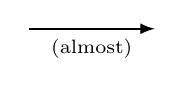
\begin{tikzpicture}
      \path[draw, -latex, thick] (-0.8,0) --node[below]  {\scriptsize (almost)} (0.8,0);
    \end{tikzpicture} &
    \begin{tabular}{c}
      \includegraphics[width=0.5\textwidth]{susyparticles_sm} \\
      {\tiny [\href{http://www.physics.gla.ac.uk/ppt/bsm.htm}{%
      http://www.physics.gla.ac.uk/ppt/bsm.htm}] }
    \end{tabular}
  \end{tabularx}
  \vspace*{-50pt}
  \begin{tabular}{VVV}
    \includegraphics[width=0.25\textwidth]{fermionloop2} &
    \hspace{15pt}
    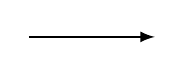
\begin{tikzpicture}
      \path[draw, -latex, thick] (-0.8,0) --node {} (0.8,0);
    \end{tikzpicture} &
    \begin{equation*}
      \parbox{20mm}{\includegraphics[width=0.2\textwidth]{fermionloop2}}
      \quad \quad \quad \, + \quad
      \parbox{20mm}{\includegraphics[width=0.2\textwidth]{scalarcubicloop} \\
        \vspace*{-5pt}
      \includegraphics[width=0.2\textwidth]{scalarquarticloop} }
    \end{equation*}
  \end{tabular}
  \vspace{30pt}
\end{frame}

\begin{frame}
  \frametitle{MSSM Field Content}
  \begin{columns}[t]
    \begin{column}{0.4\textwidth}
      \begin{itemize}\itemsep1em
        \item {\color{blue} Minimal} extension of the SM compatible with SUSY
        \item SM matter, gauge fields $\Rightarrow$ supermultiplets
        \item Additional Higgs doublet required
        \item Characterised by superpotential $+$ soft SUSY breaking
          interactions
          \begin{itemize}
            \item in general $\Rightarrow$ \alert{large number of new
              parameters}
          \end{itemize}
      \end{itemize}
    \end{column}
    \begin{column}{0.6\textwidth}
      \vspace{-40pt}
      \begin{table}[h]
        \centering
        \small
        \begin{tabular}{cccccc}
          \toprule
          & $s = 0$ & $s = \frac{1}{2}$ & $SU(3)_C$ & $SU(2)_L$
          & $\sqrt{\frac{5}{3}} Q_i^Y$ \\
          \midrule
          $\hat{Q}_i$ & $\begin{pmatrix} \tilde{u}_{L} \\
            \tilde{d}_{L} \end{pmatrix}_i$
            & $\begin{pmatrix} u_{L} \\ d_L\end{pmatrix}_i$
            & $\mathbf{3}$ & $\mathbf{2}$ & $\frac{1}{6}$ \\[1em]
          $\hat{u}^c_i$ & $\tilde{u}^*_{iR}$ & $u^c_{iR}$
            & $\bar{\mathbf{3}}$ & $\mathbf{1}$ & $-\frac{2}{3}$ \\[0.5em]
          $\hat{d}^c_i$ & $\tilde{d}^*_{iR}$ & $d^c_{iR}$
            & $\bar{\mathbf{3}}$ & $\mathbf{1}$ & $\frac{1}{3}$ \\[0.5em]
          $\hat{L}_i$ & $\begin{pmatrix} \tilde{\nu}_{L} \\
            \tilde{e}_{L} \end{pmatrix}_i$
            & $\begin{pmatrix} \nu_{L}\\ e_L \end{pmatrix}_i$
            & $\mathbf{1}$ & $\mathbf{2}$ & $-\frac{1}{2}$ \\[1em]
          $\hat{e}^c_i$ & $\tilde{e}^*_{iR}$ & $e^c_{iR}$
                        & $\mathbf{1}$ & $\mathbf{1}$ & $1$ \\[0.5em]
          $\hat{H}_d$ & $\begin{pmatrix} H_d^0 \\ H_d^- \end{pmatrix}$
            & $\begin{pmatrix} \tilde{H}_d^0 \\ \tilde{H}_d^- \end{pmatrix}$
            & $\mathbf{1}$ & $\mathbf{2}$ & $-\frac{1}{2}$ \\[1em]
          $\hat{H}_u$ & $\begin{pmatrix} H_u^+ \\ H_u^0 \end{pmatrix}$
            & $\begin{pmatrix} \tilde{H}_u^+ \\ \tilde{H}_u^0 \end{pmatrix}$
            & $\mathbf{1}$ & $\mathbf{2}$ & $\frac{1}{2}$ \\[1em]
          \bottomrule
        \end{tabular}
      \end{table}
    \end{column}
  \end{columns}
  \begin{empheq}[box=\widefbox]{equation*}
    W_{\text{MSSM}}^{\text{RPC}} = \mu ( \hat{H}_d \cdot \hat{H}_u )
      + y_{ij}^e \hat{e}^c_i ( \hat{L}_j \cdot \hat{H}_d )
      + y_{ij}^d \hat{d}^c_i ( \hat{Q}_j \cdot \hat{H}_d )
      + y_{ij}^u \hat{u}_i^c ( \hat{H}_u \cdot \hat{Q}_j )
  \end{empheq}
\end{frame}

% extra slide here showing e.g., gauge coupling unification, REWSB,
% other nice features of the model?

% continuing into DM in the MSSM (or put this later?)
\begin{frame}
  \frametitle{DM in the (RPC) MSSM}
  \begin{columns}[t]
    \begin{column}{0.5\textwidth}
  \begin{itemize} \itemsep1em
    \item Most general superpotential $\supset$ \alert{$B$, $L$ violating
      interactions}
    \item Forbid most dangerous terms? $\Rightarrow$
      impose matter parity ($\equiv$ $R$-parity):
      \begin{empheq}[box=\widefbox]{equation*}
        \color{blue} Z_2^M = (-1)^{3(B-L)}
      \end{empheq}
    \item $R$-parity conservation $\Rightarrow$ electrically neutral
      LSP is stable, natural WIMP DM candidate
    \item Standard MSSM candidate is lightest $\tilde{\chi}^0$,
      \begin{equation*}
        \tilde{\chi}_1^0 = N_{11} \tilde{H}_d^0 + N_{12} \tilde{H}_u^0
        + N_{13} \tilde{W}_3 + N_{14} \tilde{B}
      \end{equation*}
    \item Mixings $N_{1i}$ $\Rightarrow$ different DM scenarios
      (``bino-like'', ``wino-like'', $\ldots$)
  \end{itemize}
    \end{column}
    \begin{column}{0.5\textwidth}
      \begin{figure}
        \includegraphics[width=\textwidth]{gambit_cmssm_mchi0_omega}
      \end{figure}
      \begin{center}
        \tiny [\href{http://arxiv.org/abs/1705.07935}{arXiv:1705.07935}]
      \end{center}
    \end{column}
    \end{columns}
\end{frame}

\begin{frame}
  \frametitle{The "Little Hierarchy Problem"}
   \begin{figure}
      \includegraphics[width=0.75\textwidth]{higgs_mass_prl}
    \end{figure}
    \begin{center}
      MSSM tree-level prediction:
    \begin{equation*}
      m_{h_1}^2 \leq m_Z^2 \cos^2 2\beta \lesssim (91 \text{ GeV})^2
   \end{equation*}
 \end{center}
\end{frame}

\begin{frame}
  \frametitle{The "Little Hierarchy Problem"}
  \begin{itemize}\itemsep1em
    \item $m_{h_1} \approx 125$ GeV $\Rightarrow$ large higher order
      corrections
      \begin{equation*}
        m_{h_1}^2 \approx m_Z^2 \cos^2 2\beta \left ( 1 - \frac{3}{8\pi^2}
          \frac{m_t^2}{v^2} \ln \frac{m_{\tilde{t}_1} m_{\tilde{t}_2}}{M_t^2}
          \right ) {+ \color{blue} \frac{3}{4\pi^2} \frac{m_t^4}{v^2} \ln
          \frac{m_{\tilde{t}_1} m_{\tilde{t}_2}}{M_t^2}} + \ldots
      \end{equation*}
    \item $\Rightarrow$ also large corrections to prediction for $m_Z$
      at SUSY scale $M_S$:
      \begin{equation*}
        \frac{m_Z^2}{2} = -\mu^2 + \frac{\overbrace{{\color{red} m_{H_d}^2} -
          {\color{red} m_{H_u}^2}}^{\text{RGE effects}} \tan^2\beta}
          {\tan^2\beta - 1} {\color{red} +  \delta_{1-\textrm{loop}}} ,
      \end{equation*}
      \begin{equation*}
          {\color{red}
          \delta_{1-\textrm{loop}} = \frac{3}{8\pi^2} \frac{m_t^2}{v^2
            \cos 2\beta} \left [ m_{\tilde{t}_1}^2 \left ( \ln
            \frac{m_{\tilde{t}_1}^2}{M_S^2} - 1 \right ) + m_{\tilde{t}_2}^2
            \left ( \ln \frac{m_{\tilde{t}_2}^2}{M_S^2} - 1 \right ) \right ]
            + \ldots }
      \end{equation*}
    \item $\Rightarrow$ naturalness problem?
    \item \alert{$\mu$-problem}: $m_Z^2/2 = -\mu^2 + \ldots \Rightarrow \mu
      \sim$ soft parameters?
  \end{itemize}
\end{frame}

\begin{frame}
  \frametitle{The "Little Hierarchy Problem"}
  \begin{itemize}
    \item E.g., constrained models $\Rightarrow$ large \emph{sensitivities}
      $\Delta$
  \end{itemize}
  \begin{figure}
    \includegraphics[width=0.6\textwidth]{mssm_higgs_tuning}
  \end{figure}
  \vspace*{-10pt}
  \begin{center}
    {\tiny [\href{https://arxiv.org/abs/1203.0569v2}{arXiv:1203.0569}]}
  \end{center}
\end{frame}

\section{$E_6$ Inspired Models}

\begin{frame}
  \frametitle{Non-minimal SUSY Models}
  \begin{itemize} \itemsep1em
    \item Motivated by MSSM shortcomings such as LHP, $\mu$-problem
      \begin{itemize}
        \item also, e.g., non-zero $\nu$ masses, baryogenesis, $\ldots$
      \end{itemize}
    \item Extend MSSM matter content and/or gauge symmetries
    \item Simplest example: NMSSM $=$ MSSM $+$ SM singlet superfield,
      \vspace{5pt}
      \begin{figure}
        \centering
        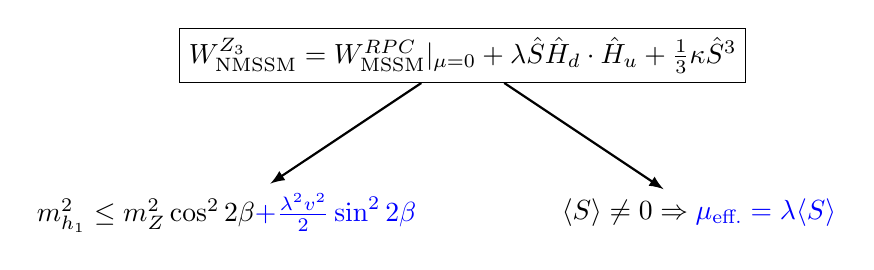
\begin{tikzpicture}[node distance=0.5cm, auto]
          \tikzstyle{arrow} = [draw, -latex, thick]

          \node[rectangle, draw, text centered] (superpotential)
            { $
                W_{\text{NMSSM}}^{Z_3} = W_{\text{MSSM}}^{RPC}|_{\mu = 0} +
                \lambda \hat{S} \hat{H}_d \cdot \hat{H}_u
                + \frac{1}{3} \kappa \hat{S}^3
              $ };
            \node[rectangle, text centered] (higgs) at (-3,-2)
            { $m_{h_1}^2 \leq m_Z^2 \cos^2 2\beta {\color{blue}
                + \frac{\lambda^2 v^2}{2} \sin^2 2\beta }$ };
              \node[rectangle, text centered] (mu) at (3,-2)
                { $\langle S \rangle \neq 0 \Rightarrow {\color{blue}
                    \mu_{\text{eff.}} = \lambda \langle S \rangle}$ };
          \path[arrow] (superpotential) -- node {} (higgs);
          \path[arrow] (superpotential) -- node{} (mu);
        \end{tikzpicture}
      \end{figure}
    \item Not without complications, may suffer from additional problems
      \begin{itemize}
        \item e.g., domain walls in the NMSSM
      \end{itemize}
  \end{itemize}
\end{frame}

\begin{frame}
  \frametitle{$U(1)$ Extensions of the MSSM}
    \begin{equation*}
      SU(3)_C \times SU(2)_L \times U(1)_Y \to
      SU(3)_C \times SU(2)_L \times U(1)_Y \times U(1)^\prime
    \end{equation*}
    \vspace{-15pt}
  \begin{columns}[t]
    \begin{column}{0.45\textwidth}
      \begin{itemize} \itemsep1em
        \item Well-motivated extensions of MSSM, NMSSM
        \item $W_{\text{USSM}} \supset \lambda \hat{S} \hat{H}_d
          \cdot \hat{H}_u$, $Q^\prime_{\hat{S}} \neq 0$ $\Rightarrow$
          $\langle S \rangle = s / \sqrt{2}$ also breaks $U(1)^\prime$,
          generating {\color{blue} massive $Z^\prime$}
        \item Consistent model requires anomaly cancellation
          \begin{itemize}
            \item either family non-universal $U(1)^\prime$ charges
              or {\color{blue} extra matter}
          \end{itemize}
        \item Additional states $\Rightarrow$ exciting phenomenology
      \end{itemize}
    \end{column}
    \begin{column}{0.6\textwidth}
      \vspace{-10pt}
      \begin{figure}
        \centering
        \includegraphics[width=\textwidth]{treelevel_higgs_upperbound_plot}
      \end{figure}
    \end{column}
  \end{columns}
\end{frame}

\begin{frame}
  \frametitle{$E_6$ Inspired Models}
  \begin{itemize} \itemsep1em
     \item Lead to $U(1)$ extended models at low-energies:
      \begin{align*}
        E_6&\longrightarrow SO(10)\times U(1)_\psi \\
        &\longrightarrow SU(5)\times U(1)_\psi\times U(1)_\chi\\
        &\longrightarrow SU(3)_C\times SU(2)_L\times U(1)_Y\times
        U(1)_\psi\times U(1)_\chi\\
        &\longrightarrow SU(3)_C\times SU(2)_L\times U(1)_Y\times
        U(1)^\prime
      \end{align*}
    \item Resulting charges $Q' = Q_\chi \cos \theta_{E_6}
      + Q_\psi \sin \theta_{E_6}$, e.g., class of models
      \begin{table}[h]
        \begin{tabular}{cl}
          $U(1)_N$: & $Q_N = Q(\theta_{E_6} = \arctan\sqrt{15})$
            ($\equiv$ E$_6$SSM) \\
          $U(1)_\psi$: & $Q_\psi = Q(\theta_{E_6} = \pi / 2)$\\
          $U(1)_\eta$: & $Q_\eta = -Q(\theta_{E_6} = \pi -
            \arctan\sqrt{5/3})$\\
          $U(1)_I$: & $Q_I = -Q(\theta_{E_6} = \arctan\sqrt{3/5})$
        \end{tabular}
      \end{table}
    \item Matter content fills complete $\mathbf{27}$ representations
      ({\color{blue} ensures anomaly cancellation})
      \begin{itemize}
        \item $\Rightarrow$ additional exotic states
      \end{itemize}
  \end{itemize}
\end{frame}

\begin{frame}
  \frametitle{The E$_6$SSM}
    \begin{columns}[t]
      \begin{column}{0.5\textwidth}
        \begin{itemize} \itemsep0.2em
        \item $\tan\theta_{E_6} = \sqrt{15}$ $\Rightarrow$ $U(1)_N$
          under which right-handed neutrinos are uncharged
          \begin{itemize}
            \item allows {\color{blue} $\nu$ masses via see-saw} and
              {\color{blue} successful baryogenesis} [1]
          \end{itemize}
        \item Extra $\hat{L}_4$, $\hat{\overline{L}}_4$ from incomplete
          $\mathbf{27}^\prime$, $\mathbf{\overline{27}}^\prime$ for gauge
          unification
        \item Low-energy matter content from $\mathbf{27}$-plet:
          \begin{align*}
            &(\hat{Q}_i, \, \hat{u}^c_i, \, \hat{d}^c_i, \, \hat{L}_i, \,
            \hat{e}^c_i) + (\hat{D}_i, \, \hat{\overline{D}}_i)\\
            &\quad {} + (\hat{S}_{i}) + (\hat{H}^u_i) + (\hat{H}^d_i)
          \end{align*}
        \item Higgs doublets $\hat{H}^d_3$, $\hat{H}^u_3$ and one singlet
          $\hat{S}_3$ get VEVs ($\Rightarrow$ EWSB and break $U(1)_N$)
          \vfill
        \end{itemize}
      \end{column}
      \begin{column}{0.5\textwidth}
        \vspace{-40pt}
        \begin{table}[h]
          \centering
          \begin{tabular}{ccccc}
            \toprule
            & $SU(3)_C$ & $SU(2)_L$ & $\sqrt{\frac{5}{3}} Q_i^Y$
            & $\sqrt{40} Q_i^N$ \\
            \midrule
            $\hat{Q}_i$ & $\mathbf{3}$ & $\mathbf{2}$ & $\frac{1}{6}$ & $1$ \\
            $\hat{u}_i^c$ & $\mathbf{\overline{3}}$ & $\mathbf{1}$
            & $-\frac{2}{3}$ & $1$ \\
            $\hat{d}_i^c$ & $\mathbf{\overline{3}}$ & $\mathbf{1}$
            & $\frac{1}{3}$ & $2$ \\
            $\hat{L}_i$ & $\mathbf{1}$ & $\mathbf{2}$ & $-\frac{1}{2}$ & $2$ \\
            $\hat{e}_i^c$ & $\mathbf{1}$ & $\mathbf{1}$ & $1$ & $1$ \\
            $\hat{S}_i$ & $\mathbf{1}$ & $\mathbf{1}$ & $0$ & $5$ \\
            $\hat{H}_i^u$ & $\mathbf{1}$ & $\mathbf{2}$ & $\frac{1}{2}$
            & $-2$ \\
            $\hat{H}_i^d$ & $\mathbf{1}$ & $\mathbf{2}$ & $-\frac{1}{2}$
            & $-3$ \\
            $\hat{D}$ & $\mathbf{3}$ & $\mathbf{1}$ & $-\frac{1}{3}$ & $-2$ \\
            $\hat{\overline{D}}$ & $\mathbf{\overline{3}}$ &  $\mathbf{1}$
            & $\frac{1}{3}$ & $-3$ \\
            $\hat{L}_4$ & $\mathbf{1}$ & $\mathbf{2}$ & $-\frac{1}{2}$ & $2$ \\
            $\hat{\overline{L}}_4$ & $\mathbf{1}$ & $\mathbf{\overline{2}}$
            & $\frac{1}{2}$ & $-2$ \\
            \bottomrule
          \end{tabular}
        \end{table}
      \end{column}
    \end{columns}
    \vspace{-4pt}
    \begin{align*}
      \Aboxed{W_{\text{E}_6\text{SSM}} \approx y_{\tau} \hat{L}_3 \cdot
        \hat{H}^d_3 \hat{e}^c_3 + y_b \hat{Q}_3 \cdot \hat{H}^d_3 \hat{d}_3^c
        + y_t \hat{H}^u_3 \cdot \hat{Q}_3 \hat{u}_3^c + \lambda_i \hat{S}_3
        \hat{H}_i^d \cdot \hat{H}_i^u  + \kappa_i \hat{S}_3 \hat{D}_i
        \hat{\overline{D}}_i + \mu_L \hat{L}_4 \cdot \hat{\overline{L}}_4}
    \end{align*}
        {\tiny [1] S.~F.~King, S.~Moretti, and R.~Nevzorov,
          \href{http://dx.doi.org/10.1103/PhysRevD.73.035009}{Phys.~Rev.~D
            \textbf{73}, 035009 (2006)}
          (\href{http://arxiv.org/abs/hep-ph/0510419}{hep-ph/0510419})}
\end{frame}

\section{Fine Tuning in $E_6$ Models}

\begin{frame}
  \frametitle{The Impact of $D$-terms}
  \begin{columns}[t]
    \begin{column}{0.5\textwidth}
      { \small
      \begin{equation*}
        m_{h_1}^2 \leq m_Z^2 \cos^2 2\beta + \frac{\lambda^2 v^2}{2}
        \sin^2 2\beta {\color{blue} + \frac{m_Z^2}{4} \left (1 + \frac{1}{4}
        \cos 2\beta \right )^2}
      \end{equation*}}
      \begin{itemize} \itemsep1em
        \item Extra $D$-terms $\Rightarrow$ reduced radiative corrections
        \item E.g., CE$_6$SSM shows reduced sensitivity compared to CMSSM
      \end{itemize}
      \begin{figure}
        \centering
        \includegraphics[width=0.5\textwidth]{ce6ssm_tuning}
        \includegraphics[width=0.5\textwidth]{ce6ssm_higgs_mass}
      \end{figure}
      \vspace*{-25pt}
      \begin{center}
        {\tiny [\href{https://arxiv.org/abs/1302.5291}{arXiv:1302.5291}]}
      \end{center}
    \end{column}
    \begin{column}{0.5\textwidth}
      { \small
      \begin{equation*}
        c \frac{m_Z^2}{2} \approx -\mu_{\text{eff.}}^2
          + \frac{\bar{m}_{H_d}^2 - \bar{m}_{H_u}^2 \tan^2\beta}
          {\tan^2\beta - 1} {\color{red} + d \frac{m_{Z'}^2}{2}}
      \end{equation*}}
      \begin{itemize} \itemsep1em
        \item Large $m_{Z^\prime}$ $\Rightarrow$ \alert{large
          contribution to $m_Z$}
        \item $m_{Z^\prime} \gg m_Z$ $\Rightarrow$ fine-tuning again?
        \item Coefficient $d = d(\tan\beta; \theta_{E_6})$ $\Rightarrow$
          impact of $m_{Z^\prime}$ depends on $\theta_{E_6}$
          \begin{itemize}
            \item $c = c(\tan\beta; \theta_{E_6}) = O(1)$
          \end{itemize}
      \end{itemize}
      \begin{figure}
        \centering
        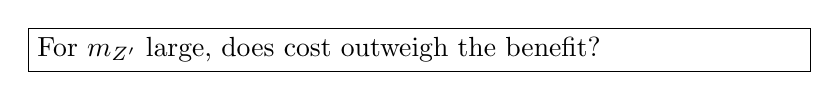
\begin{tikzpicture}[node distance=2cm,auto]
          \node[rectangle,draw,text width=0.8\columnwidth] (question)
            {For $m_{Z^\prime}$ large,
              does cost outweigh the benefit?};
        \end{tikzpicture}
      \end{figure}
    \end{column}
  \end{columns}
\end{frame}

\begin{frame}
  \frametitle{Model Dependent Contributions}
  \begin{itemize} \itemsep1em
    \item Radiative contributions, e.g.,
      \begin{equation*}
        m_{H_u}^2(M_S) \sim m_{H_u}^2(M_X) {\color{red}
          + \frac{3 y_t^2}{8\pi^2}
          [ m_{H_u}^2(M_X) + m_{Q_3}^2(M_X) + A_t^2(M_X) ] \ln \frac{M_S}{M_X}
          } + \ldots
      \end{equation*}
      depend on
      \begin{itemize}
        \item soft SUSY breaking mechanism ($\Leftrightarrow$ values of
          $m_{H_u}^2(M_X)$, $m_{Q_3}^2(M_X)$, etc.)
        \item scale of SUSY breaking, $M_X$
      \end{itemize}
    \item I.e., conclusions strongly depend on assumptions about (unknown)
      high-energy boundary conditions
    \item Contrast with \emph{tree-level} $m_{Z^\prime}$ effect
    \item Study models at low energies $\Rightarrow$ {\color{blue}
        conservative picture of tuning}
    \item Alternative: {\color{orange} measure fine-tuning} purely in terms
      of low-energy parameters?
  \end{itemize}
\end{frame}

\begin{frame}
  \frametitle{Measuring Fine-tuning?}
  \begin{center}
    What constitutes "fine-tuning"? \\
    Opinions differ.
  \end{center}
  \begin{itemize} \itemsep1em
    \item Large cancellations?
      \begin{equation*}
        \Delta_{EW} = \max_i \frac{2|C_i|}{m_Z^2}, \quad C_1 = -\mu^2, \,
        C_2 = \frac{m_{H_d}^2}{\tan^2\beta - 1}, \ldots
      \end{equation*}
    \item Extreme sensitivities?
      \begin{equation*}
        \Delta_{BG} = \max_i \left | \frac{\partial \ln m_Z^2}
        {\partial \ln p_i} \right | , \quad p_i \in \{\text{fundamental
        parameters}\}
      \end{equation*}
    \item High or low energy contributions ($\Delta_{EW}$ or $\Delta_{HS}$)?
      Definition of parameters $p_i$? Just $m_Z$?
    \item Model fine-tuned $\Leftrightarrow \Delta_{EW/HS/BG/\ldots} > ?$
    \item Compare tuning between models?
  \end{itemize}
\end{frame}

\begin{frame}
  \frametitle{A Bayesian Approach}
  \begin{itemize}\itemsep1em
    \item Rigorous framework {\color{blue} automatically captures intuition
      about "naturalness"}
    \item Bayes' theorem applied to model $M$, parameters $\bm{x}$,
      "observables" $\bm{O}$:
      \begin{gather*}
        p(\bm{x}|\text{data},M) = \frac{p(\text{data}|\bm{x},M) p(\bm{x}|M)}
        {p(\text{data}|M)} , \quad
        p(M|\text{data}) = \frac{p(\text{data}|M) p(M)}{p(\text{data})} \\
        {\color{orange} p(\text{data}|M)}
      = \int d^n x_i\; p(\text{data}|
        \bm{x},M) p(\bm{x}|M), \quad
        {\color{green} p_{\text{eff.}}(x_j,\ldots)} = \int dO_i \;
          p(\bm{O}, \bm{x}^\prime | M, O_i^{\text{exp.}})
      \end{gather*}
    \item Reparameterise in favour of $\bm{O}$, e.g.,
      \begin{equation*}
        p(\bm{x}|M) = \mathcal{J} p(\bm{O},\bm{x}^\prime|M)
      \end{equation*}
      $\Rightarrow$ {\color{orange} evidence} and {\color{green}
      effective priors} {\color{blue} suppressed by Jacobian} $\Delta_J
      \sim \mathcal{J}$,
      \begin{equation*}
        \Delta_J = \left | \det \frac{\partial \ln O_i}{\partial \ln x_j}
        \right |
      \end{equation*}
 \end{itemize}
\end{frame}

\begin{frame}
  \frametitle{Example: Bayesian Naturalness in the NMSSM}
  \begin{columns}[t]
    \begin{column}{0.6\textwidth}
      \vspace*{-30pt}
      \begin{columns}[t]
        \begin{column}{0.5\textwidth}
          \begin{figure}
            \centering
            \includegraphics[width=1.1\textwidth]{CNMSSM_BG_m0m12}
          \end{figure}
        \end{column}
        \begin{column}{0.5\textwidth}
          \begin{figure}
            \centering
            \includegraphics[width=1.1\textwidth]{CNMSSM_GUT_J_m0m12}
          \end{figure}
        \end{column}
      \end{columns}
      \vspace{10pt}
      \begin{minipage}[t][5cm][t]{\textwidth}
      \begin{itemize} \itemsep1em
        \item $\Delta_{BG}$, $\Delta_J$ qualitatively similar
        \item High posterior density $\Leftrightarrow$ low fine-tuning
        \item Before $m_{h_1} \approx 125$ GeV, weak-scale soft parameters
          preferred
      \end{itemize}
    \end{minipage}
    \end{column}
    \begin{column}{0.35\textwidth}
      \begin{figure}
        \centering
        \includegraphics[width=\textwidth]{CNMSSM_pdf_mz_m0m12}
      \end{figure}
      \vspace*{-20pt}
      \begin{center}
        {\tiny [\href{https://arxiv.org/abs/1709.07895}{arXiv:1709.07895}]}
      \end{center}
    \end{column}
  \end{columns}
\end{frame}

\begin{frame}
  \frametitle{Example: Bayesian Naturalness in the NMSSM}
  \begin{columns}[t]
    \begin{column}{0.6\textwidth}
      \vspace*{-30pt}
      \begin{columns}[t]
        \begin{column}{0.5\textwidth}
          \begin{figure}
            \centering
            \includegraphics[width=1.1\textwidth]{CNMSSM_BG_mh_m0m12}
          \end{figure}
        \end{column}
        \begin{column}{0.5\textwidth}
          \begin{figure}
            \centering
            \includegraphics[width=1.1\textwidth]{CNMSSM_GUT_J_mh_m0m12}
          \end{figure}
        \end{column}
      \end{columns}
      \vspace{10pt}
      \begin{minipage}[t][5cm][t]{\textwidth}
      \begin{itemize} \itemsep1em
        \item Inclusion of $m_{h_1} \approx 125$ GeV $\Rightarrow$
          increased $\Delta_{BG}$, $\Delta_J$
        \item Some quantitative differences, e.g., focus point
        \item Bayesian analysis consistent with intuitive tuning measures
      \end{itemize}
    \end{minipage}
    \end{column}
    \begin{column}{0.35\textwidth}
      \begin{figure}
        \centering
        \includegraphics[width=\textwidth]{CNMSSM_pdf_mz_mh_m0m12}
      \end{figure}
      \vspace*{-20pt}
      \begin{center}
        {\tiny [\href{https://arxiv.org/abs/1709.07895}{arXiv:1709.07895}]}
      \end{center}
    \end{column}
  \end{columns}
\end{frame}

\begin{frame}
  \frametitle{Fine Tuning in the E$_6$SSM}
  \begin{itemize} \itemsep1em
    \item Use $\Delta_{BG}$ for simplicity and comparison with
      previous results
      \begin{itemize}
        \item {\color{blue} Expect similar conclusions to full Bayesian
          approach}
      \end{itemize}
    \item Fundamental model parameters $\Leftrightarrow$ boundary values at
      $M_X$
      \begin{itemize}
        \item e.g. $m_{H_u}^2(M_X)$, $A_t(M_X)$, $A_\lambda(M_X)$, $M_3(M_X)$,
          $\ldots$
      \end{itemize}
    \item Minimise impact of high-energy assumptions $\Rightarrow$ choose
      low $M_X = 20$ TeV
    \item Account for remaining impact with approximate solutions
      ($t = \ln \frac{M_S}{M_X}$, $\frac{\mathrm{d}p}{\mathrm{d}t} =
      \frac{\beta_p^{(1)}}{\left ( 4\pi\right )^2}
      + \frac{\beta_p^{(2)}}{\left (4\pi \right )^4}$)
      \begin{equation*}
        p (M_S) \approx p(M_X) + \frac{t}{\left ( 4 \pi \right )^2}
          \left ( \beta_p^{(1)} (M_X) + \frac{1}{\left ( 4\pi \right )^2}
          \beta_p^{(2)}(M_X) \right ) + \frac{t^2}{2\left ( 4\pi \right )^4}
          \sum_{\{q\}} \beta_q^{(1)}(M_X) \left . \frac{\partial
          \beta_p^{(1)}}{\partial q} \right |_{M_X}
      \end{equation*}
    \item Dependence of $\Delta_{BG}$ on $m_{Z^\prime}$?
  \end{itemize}
\end{frame}

\begin{frame}
  \frametitle{Numerical Methods}
  \begin{columns}
    \begin{column}{0.6\textwidth}
      \begin{itemize} \itemsep1em
        \item Consider multiple $\theta_{E_6}$ values ({\color{blue}
          role of $d$ coefficient?})
        \item "Phenomenological" boundary conditions at $M_X$ $\Rightarrow$
          compute tunings for
          \begin{align*}
            p &= \{ \lambda, A_\lambda, m_{H_d}^2, m_{H_u}^2, m_S^2,
              m_{Q_3}^2, m_{u_3^c}^2, A_t,\\
            & \quad \quad {} M_1, M_2, M_3, M_1' \}
          \end{align*}
        \item 2-loop RGEs generated by
          \href{https://sarah.hepforge.org/}{SARAH} $+$
          \href{https://flexiblesusy.hepforge.org/}{FlexibleSUSY}
        \item For MSSM used modified
          \href{http://softsusy.hepforge.org/}{SOFTSUSY} 3.3.10
          \begin{itemize}
            \item Assume pMSSM boundary conditions with $\mu, B \in [-1,1]$
              TeV
          \end{itemize}
        \item Neglect kinetic mixing
          \begin{itemize}
            \item small in models considered
            \item \alert{not negligible in general (e.g. $U(1)_{B-L}$)}
          \end{itemize}
      \end{itemize}
    \end{column}
    \begin{column}{0.4\textwidth}
      \vspace*{-20pt}
      \begin{table}[h]
        \centering
        \begin{tabulary}{\textwidth}{C}
          \toprule
          $2 \leq \tan\beta \leq 50$ for $U(1)_N$, \\
          $\tan\beta = 10$ for all others \\
          \midrule
          $-3 \leq \lambda \leq 3$\\
          \midrule
          $-10\textrm{ TeV } \leq A_\lambda \leq 10\textrm{ TeV}$ \\
          \midrule
          $ 200 \textrm{ GeV } \leq m_{Q_3} \leq 2000 \textrm { GeV}$\\
          \midrule
          $ 200 \textrm{ GeV } \leq m_{u_3} \leq 2000 \textrm { GeV}$\\
          \midrule
          $-10 \textrm{ TeV } \leq A_t \leq 10 \textrm { TeV}$\\
          \midrule
          $M_2=100\textrm{ GeV, } 1050\textrm{ GeV, } 2000 \textrm{ GeV}$ \\
          \bottomrule
        \end{tabulary}
      \end{table}
      \begin{itemize}
        \item Other soft scalar masses $= 5$ TeV, $M_1 = M_1' = 300$ GeV,
          $M_3 = 2$ TeV
      \end{itemize}
    \end{column}
  \end{columns}
\end{frame}

\begin{frame}
  \frametitle{High-scale Model Dependence}
  \begin{columns}
    \begin{column}{0.5\textwidth}
      \begin{itemize}
        \item $\Delta_{BG}$ highly model-dependent
          \begin{itemize}
            \item E.g., E$_6$SSM BM1 (unconstrained) vs. BM2 ($\sim$
              CE$_6$SSM)
          \end{itemize}
      \end{itemize}
      \vspace*{-15pt}
      \begin{figure}
        \begin{center}
          \includegraphics[width=\textwidth]
            {e6ssm_mssm_benchmark_points_tuning_vs_cutoff_bw_var}
        \end{center}
      \end{figure}
      \begin{center}
        \tiny [\href{https://arxiv.org/abs/1503.08929}{arXiv:1503.08929}]
      \end{center}
    \end{column}
    \begin{column}{0.5\textwidth}
      \vspace*{-20pt}
      \begin{figure}
        \begin{center}
          \includegraphics[width=\textwidth]{%
          e6ssm_light_zprime_BM1_all_tuning_data_bw_var}
        \end{center}
      \end{figure}
      \begin{itemize} \itemsep1em
        \item Large $M_X$ $\Rightarrow$ RG contributions (e.g., $M_3$ in
          E$_6$SSM BM1) are dominant
        \item High-scale models: impact of $m_{Z^\prime}$ limits not easily
          seen
      \end{itemize}
    \end{column}
  \end{columns}
\end{frame}

\begin{frame}
  \frametitle{$U(1)_N$: $Q_N = Q(\theta_{E_6} = \arctan \sqrt{15})$,
    $d(\tan\beta = 10) \approx 0.40$}
  \begin{columns}
    \begin{column}{0.5\textwidth}
      \vspace*{-15pt}
      \begin{figure}
        \includegraphics[width=1.2\textwidth]{%
          all_models_tuning_vs_higgs_bw_var}
      \end{figure}
      \begin{center}
        \tiny [\href{https://arxiv.org/abs/1503.08929}{arXiv:1503.08929}]
      \end{center}
    \end{column}
    \begin{column}{0.5\textwidth}
      \begin{itemize} \itemsep1.5em
        \item Low $M_X$ $\Rightarrow$ $\tilde{t}$ tuning reduced
        \item {\color{blue} $m_{Z^\prime}$ sets lower limit on $\Delta_{BG}$}
          \begin{itemize}
            \item $\Rightarrow$ conservative limit on naturalness in E$_6$SSM
          \end{itemize}
        \item $m_{Z'} \approx 2.5$ TeV (\alert{old limit!})
          $\Rightarrow$ minimum tuning already exceeds MSSM
          \begin{itemize}
            \item $\approx$ equivalent to MSSM with $\geq 700$ GeV
              $\tilde{\chi}^\pm$ ($\Rightarrow$ lower bound on $\mu$)
          \end{itemize}
        \item \alert{Warning: only 1-loop $t$, $\tilde{t}$ + leading 2-loop
            Higgs mass calculation $\Rightarrow$ large Higgs mass uncertainty}
      \end{itemize}
    \end{column}
  \end{columns}
\end{frame}

\begin{frame}
  \frametitle{$U(1)_\psi$: $Q_\psi = Q(\theta_{E_6} = \pi / 2)$,
    $d(\tan\beta = 10) \approx 0.50$}
  \begin{columns}
    \begin{column}{0.5\textwidth}
      \vspace*{-15pt}
      \begin{figure}
        \includegraphics[width=1.2\textwidth]{%
          e6psi_tb10_tuning_vs_higgs_bw_var}
      \end{figure}
      \begin{center}
        \tiny [\href{https://arxiv.org/abs/1503.08929}{arXiv:1503.08929}]
      \end{center}
    \end{column}
    \begin{column}{0.5\textwidth}
      \begin{itemize} \itemsep1.5em
        \item {\color{blue} Minimum $\Delta_{BG}$ depends on $\theta_{E_6}$}
          \begin{itemize}
            \item $\Rightarrow$ size of tuning depends on low-energy $U(1)$
          \end{itemize}
        \item E.g., $U(1)_\psi$, $d \approx 0.5$ compared to $\approx 0.4$
          in E$_6$SSM
        \item $\Rightarrow$ lower bound for given $m_{Z^\prime}$ increased
        \item $d \neq 0$ $\Rightarrow$ $m_{Z^\prime}$ still sets minimal
          sensitivity
      \end{itemize}
    \end{column}
  \end{columns}
\end{frame}

\begin{frame}
  \frametitle{$U(1)_\eta$: $Q_\eta = -Q(\theta_{E_6} = \pi
    - \arctan\sqrt{5/3})$, $d(\tan\beta = 10) \approx 0.81$}
  \begin{columns}
    \begin{column}{0.5\textwidth}
      \vspace*{-15pt}
      \begin{figure}
        \includegraphics[width=1.2\textwidth]{%
          e6eta_tb10_tuning_vs_higgs_bw_var}
      \end{figure}
      \begin{center}
        \tiny [\href{https://arxiv.org/abs/1503.08929}{arXiv:1503.08929}]
      \end{center}
    \end{column}
    \begin{column}{0.5\textwidth}
      \begin{itemize} \itemsep1.5em
        \item Largest $D$-term contribution, $d \approx 0.81$
        \item \alert{$\Rightarrow$ largest tuning for given $m_{Z^\prime}$}
          \begin{itemize}
            \item Minimum $\Delta_{BG}$ substantially larger than in $U(1)_N$,
              $U(1)_\psi$
          \end{itemize}
        \item Current $m_{Z^\prime}$ limits $\Rightarrow$ models with large
            $D$-terms already "moderately" tuned
        \item Severity of tuning depends strongly on $\theta_{E_6}$
          (i.e. charges)
      \end{itemize}
    \end{column}
  \end{columns}
\end{frame}

\begin{frame}
  \frametitle{$U(1)_I$: $Q_I = -Q(\theta_{E_6} = \arctan\sqrt{3/5})$,
    $d(\tan\beta = 10) \approx -0.01$}
  \begin{columns}
    \begin{column}{0.5\textwidth}
      \vspace*{-15pt}
      \begin{figure}
        \includegraphics[width=1.2\textwidth]{%
          e6inert_tb10_tuning_vs_higgs_bw_var}
      \end{figure}
      \begin{center}
        \tiny [\href{https://arxiv.org/abs/1503.08929}{arXiv:1503.08929}]
      \end{center}
    \end{column}
    \begin{column}{0.5\textwidth}
      \begin{itemize} \itemsep1.5em
        \item Example of model with suppressed $D$-terms
          ($Q_{H_u} = 0$)
        \item {\color{blue} $\Rightarrow$ $m_{Z^\prime}$ sensitivity much
          reduced}
        \item \alert{Trade-off: suppresses $D$-term contribution to
          $m_{h_1}$:}
          \begin{align*}
            m_{h_1}^2 &\lesssim m_Z^2 \cos^2 2\beta + \frac{\lambda^2}{2} v^2
              \sin^2 2\beta \\
              &{} {\color{red} + g_1'^2 v^2 ( Q_{H_d} \cos^2\beta +
            \underbrace{Q_{H_u} \sin^2\beta}_{=0} )^2}
          \end{align*}
        \item For current $m_{Z^\prime}$ limits, tuning is MSSM-like
      \end{itemize}
    \end{column}
  \end{columns}
\end{frame}

\section{The SE$_6$SSM}

\begin{frame}
  \frametitle{E$_6$SSM: $M_{Z^\prime} \sim M_S$}
  \begin{columns}[t]
    \begin{column}{0.5\textwidth}
      \vspace{-20pt}
      \begin{figure}
        \hspace*{-15pt}
        \includegraphics[width=7.5cm]{atlas_z_prime}
      \end{figure}
    \vspace{-22pt}
    \begin{center}
      \tiny [\href{http://arxiv.org/abs/1707.02424}{arXiv:1707.02424}]
    \end{center}
    \end{column}
    \begin{column}{0.5\textwidth}
      \vspace{-20pt}
      \begin{figure}
        \hspace*{-15pt}
        \includegraphics[width=7.5cm]{atlas_cmssm}
      \end{figure}
      \vspace{-11pt}
      \begin{center}
        \tiny [\href{http://arxiv.org/abs/1507.05525}{arXiv:1507.05525}]
      \end{center}
    \end{column}
  \end{columns}
\end{frame}

\begin{frame}
  \frametitle{E$_6$SSM: Discrete Symmetries}
  \begin{itemize}\itemsep0.8em
  \item Most general superpotential
    \begin{equation*}
      W \supset {\color{red} g_{ijk}^D} \hat{D}_i \hat{Q}_j \cdot \hat{Q}_k
      + {\color{red} \tilde{g}_{ijk}^E} \hat{e}_i^c \hat{D}_j \hat{u}_k^c
      + {\color{orange} y_{ijk}^U} \hat{u}_i^c \hat{H}_{uj} \cdot \hat{Q}_k
      + {\color{orange} y_{ijk}^D} \hat{d}_i^c \hat{Q}_j \cdot
      \hat{H}_{dk} + \ldots
    \end{equation*}
    $\Rightarrow$ {\color{red} unacceptable $B$, $L$ violation} and
        {\color{orange} large FCNCs}
      \item Impose
        \begin{itemize}
          \item either exact $Z_2^L$ or exact $Z_2^B$ to forbid
            $B$, $L$ violating couplings
          \item approximate $Z_2^H$ to suppress FCNCs
        \end{itemize}
    \item Resulting Higgs, singlet couplings
      \begin{equation*}
        \lambda_{ijk} \hat{S}_i \hat{H}_{dj} \cdot \hat{H}_{uk}
        \rightarrow \lambda \hat{S} \hat{H}_{d3} \cdot \hat{H}_{u3}
        + \lambda_{\alpha\beta} \hat{S} \hat{H}_{d\alpha} \cdot
        \hat{H}_{u\beta} + \tilde{f}_{\alpha\beta} \hat{S}_\alpha
        \hat{H}_{d\beta} \cdot \hat{H}_{u3} + f_{\alpha\beta}
        \hat{S}_\alpha \hat{H}_{d3} \cdot \hat{H}_{u\beta}
      \end{equation*}
      $\Rightarrow$ LSP, NSLP is a (ruled out) ``inert'' neutralino
    \item Simplest viable models impose \emph{another} exact $Z_2^S$
    \item \alert{None of these $Z_2$ symmetries commute with $E_6$}
  \end{itemize}
\end{frame}

\begin{frame}
  \frametitle{The SE$_6$SSM}
  \begin{itemize} \itemsep1em
    \item $E_6$ inspired model arising from 5D or 6D orbifold GUT [2]
    \item Complete $\mathbf{27}$-plets supplemented by components
      of {\color{orange} extra $\mathbf{27^\prime}$-,
        $\mathbf{\overline{27}^\prime}$-plets}
    \item Stabilise Higgs potential $\Rightarrow$ pure singlet $\hat{\phi}$

    \item $U(1)_\psi \times U(1)_\chi \rightarrow U(1)_N \times Z_2^M$
      at intermediate scale $\Rightarrow$ {\color{blue} automatically conserved
      $Z_2^M$}
    \item Dangerous $B$, $L$ violating operators, FCNCs forbidden by
      {\color{blue} single exact $\tilde{Z}_2^H$}
  \end{itemize}
  \vspace*{8pt}
  \begin{empheq}[box=\widefbox]{align*}
    W_{\text{SE}_6\text{SSM}} = {} & \, \lambda {\color{orange} \hat{S}}
    ({\color{orange}\hat{H}_d} \cdot {\color{orange} \hat{H}_u})
    - \sigma \hat{\phi} {\color{orange}\hat{S}}
    {\color{orange}\hat{\overline{S}}}
    + \frac{\kappa}{3}\hat{\phi}^3 + \frac{\mu}{2}\hat{\phi}^2
    + \Lambda_F\hat{\phi} + \lambda_{\alpha\beta} {\color{orange}\hat{S}}
    (\hat{H}^d_{\alpha} \cdot \hat{H}^u_{\beta}) \\
    & {} + \kappa_{ij} {\color{orange}\hat{S}}
    \hat{D}_{i} \hat{\overline{D}}_{j}
    + \tilde{f}_{i\alpha} \hat{S}_{i} ({\color{orange}\hat{H}_u} \cdot
    \hat{H}^d_{\alpha}) + f_{i\alpha} \hat{S}_{i} (\hat{H}^u_{\alpha}
    \cdot {\color{orange}\hat{H}_d})
    + g^D_{ij} (\hat{Q}_i \cdot {\color{orange}\hat{L}_4})
    \hat{\overline{D}}_j \\
    & {} + h^E_{i\alpha} \hat{e}^c_{i} (\hat{H}^d_{\alpha} \cdot
    {\color{orange}\hat{L}_4})
    + \mu_L({\color{orange}\hat{L}_4} \cdot
    {\color{orange}\hat{\overline{L}}_4}) + \tilde{\sigma}
    \hat{\phi} ({\color{orange}\hat{L}_4} \cdot
    {\color{orange}\hat{\overline{L}}_4})
    + W_{\text{MSSM}}(\mu=0)
  \end{empheq}
  \vfill
  {\tiny [2] R.~Nevzorov,
        \href{http://dx.doi.org/10.1103/PhysRevD.87.015029}
             {Phys. Rev. \textbf{D} 87, 015029 (2013)}
             (\href{http://arxiv.org/abs/1205.5967}{arXiv:1205.5967})}
\end{frame}

\begin{frame}
  \frametitle{EWSB in the SE$_6$SSM}
  \begin{itemize}\itemsep1em
  \item At physical minimum,
    \begin{equation*}
      \langle H_d^0 \rangle = \frac{v_1}{\sqrt{2}} \, , \quad
      \langle H_u^0 \rangle = \frac{v_2}{\sqrt{2}} \, , \quad
      \langle S \rangle = \frac{s_1}{\sqrt{2}} \, , \quad
      \langle \overline{S} \rangle = \frac{s_s}{\sqrt{2}} \, , \quad
      \langle \phi \rangle = \frac{\varphi}{\sqrt{2}}
    \end{equation*}
  \item $S$, $\overline{S}$ develop along nearly $D$-flat direction
    $\langle S \rangle = \langle \overline{S} \rangle$ with
    \begin{equation*}
      \langle S \rangle \approx \langle \overline{S} \rangle
              {\color{blue} \sim \frac{M_S}{\sigma}}
    \end{equation*}
  \item Small $\sigma$ $\Rightarrow$ $M_{Z^\prime}^2 \sim g_1^{\prime 2} Q_S^2
    (s_1^2 + s_2^2)$ far heavier than $M_S$
  \item $\therefore$ can have $M_{Z^\prime}$ far above limits while keeping
    sparticles (relatively) light
  \item $D$-term contribution to EW scale also suppressed:
    \begin{equation*}
    c \frac{M_Z^2}{2}
    \approx -\frac{\lambda^2 s_1^2}{2} + \frac{m_{H_d}^2 -
      m_{H_u}^2 \tan^2\beta} {\tan^2\beta - 1} + d
      {\color{blue} \frac{g_1'^2 Q_S^2 (s_1^2 - s_2^2)}{2}}
    \end{equation*}
  \end{itemize}
\end{frame}

\begin{frame}
  \frametitle{Dark Matter Candidates?}
  \vspace{10pt}
  \begin{columns}
    \begin{column}{0.6\textwidth}
      \begin{itemize} \itemsep1.2em
      \item Conserved $Z_2^M$, $\tilde{Z}_2^H$ $\Rightarrow$
        \emph{two} (distinct) DM candidates
        \item ``Exotics'' $\equiv Z_2^E$ odd states, where
          $\tilde{Z}_2^H = Z_2^M \times Z_2^E$
      \item $Z_2^E$ conserved $\Rightarrow$ lightest exotic is stable
      \item Limits from exotic Higgs decays, DM direct detection
        $\Rightarrow$ inert singlinos $\tilde{S}_i$ form subdominant hot DM,
        $m_{\tilde{S}_i} \ll 1$ eV
      \item $M_{Z'} \gg M_S \gg M_Z$ $\Rightarrow$ {\color{orange}
        singlet dominated $\tilde{\chi}^0$'s} decouple
      \item $\Rightarrow$ account for $\Omega h^2$ with
        {\color{blue} MSSM-like $\tilde{\chi}_1^0$}?
      \end{itemize}
    \end{column}
    \begin{column}{0.4\textwidth}
      \begin{table}[ht]
        \centering
        \small
        \begin{tabular}{cccc}
          \toprule
          & $\tilde{Z}_2^H$ & $Z_2^M$ & $Z_2^E$ \\
          \midrule
          $\hat{Q}_i$, $\hat{u}_i^c$, $\hat{d}_i^c$, $\hat{L}_i$, $\hat{e}_i^c$,
          $\hat{N}_i^c$ & $-$ & $-$ & $+$ \\
          $\hat{H}_{\alpha}^u$, $\hat{H}_{\alpha}^d$, $\hat{S}_i$,
          $\hat{D}_i$, $\hat{\overline{D}}_i$ & $-$ & $+$ & $-$ \\
          $\hat{H}_u$, $\hat{H}_d$ & $+$ & $+$ & $+$ \\
          $\hat{S}$, $\hat{\overline{S}}$ & $+$ & $+$ & $+$ \\
          $\hat{L}_4$, $\hat{\overline{L}}_4$ & $+$ & $-$ & $-$ \\
          \bottomrule
        \end{tabular}
      \end{table}
      \vspace{8pt}
      Enlarged ($8 \times 8$) $\tilde{\chi}^0$ sector:
      \begin{center}
        $
        \qquad \large
        M_{\tilde{\chi}^0} = \begin{pmatrix}
          {\color{blue} A} & C^T \\
          C & {\color{orange} B}
        \end{pmatrix}
        $
      \end{center}
    \end{column}
  \end{columns}
\end{frame}

\begin{frame}
  \frametitle{The CSE$_6$SSM}
  \begin{itemize}
    \vfill
    \item {\color{red} General model is complicated}
          \begin{itemize}
            \item $O(200)$ new parameters (assuming no new sources of
                  CP-violation)
            \item Many masses and mixings
          \end{itemize}
    \vfill
    \item Consider constrained model (CSE$_6$SSM) inspired by gravity
          mediated SUSY breaking
    \vfill
  \item {\color{blue} Universal soft breaking parameters: $M_{1/2}$, $A_0$,
    $B_0$, $m_0$}
    \vfill
    \item Interested in mechanism decoupling $Z^\prime$ from EWSB conditions
          $\Rightarrow$ can have large $s = \sqrt{s_1^2 + s_2^2}$
    \vfill
    \item Higgsino mass set by $\mu_{\text{eff}} = \lambda s_1 / \sqrt{2}$
      $\Rightarrow$ acceptable LSP mass ($\lesssim$ TeV) for small
      $\lambda$
    \vfill
    \item $\Rightarrow$ other exotic couplings must be small,
          otherwise exotic states are tachyonic
  \end{itemize}
\end{frame}

\begin{frame}
  \frametitle{Parameter Space Scans}
  \begin{itemize}\itemsep1em
    \item Focus on heavy $Z^\prime$, $s = 650$ TeV, choose fixed
      $\mu_{\text{eff}}$
    \item Achieve using semi-analytic solutions for soft parameters:
      \begin{align*}
        M_i(Q) &= p_i(Q) M_{1/2} + q_i(Q) A_0 \, , \quad
        A_i(Q) = e_i(Q) A_0 + f_i(Q) M_{1/2} \, , \\
        m_i^2(Q) &= a_i(Q) m_0^2 + b_i(Q) M_{1/2}^2 + c_i(Q) A_0 M_{1/2}
        + d_i(Q) A_0^2 \, , \, \ldots
      \end{align*}
    \item Fix $m_0$ from EWSB,
      $m_0^2 \sim -\frac{b_{H_u}}{a_{H_u}} M_{1/2}^2 - \ldots$
    \item Implemented in FlexibleSUSY for {\color{blue} full 1-loop masses
      and 2-loop RGEs}
      \begin{itemize}
      \item Resulting ``semi-analytic solver'' forms part of
        FlexibleSUSY 2.0 [3], along with many other updates.
      \end{itemize}
    \item Require $\Omega h^2 \leq 0.1187$ (micrOMEGAs) and
      $m_{h_1} = 125.09 \pm 3$ GeV
    \item Compare with CMSSM for $|\mu| \sim 400$ GeV and $|\mu| \sim
      1$ TeV
  \end{itemize}
  \vfill
      {\tiny [3] P.~Athron, M.~Bach, D.~Harries, T.~Kwasnitza,
        J.-h.~Park, D.~St\"{o}ckinger, A.~Voigt, and J.~Ziebell,
        \href{http://arxiv.org/abs/1710.03760}{arXiv:1710.03760}
      }
\end{frame}

\section{Dark Matter in the CSE$_6$SSM}

\begin{frame}
  \frametitle{Sparticle Mass Spectrum}
  \begin{columns}[t]
    \begin{column}{0.4\textwidth}
      \vspace{-30pt}
      \begin{figure}
        \begin{center}
          \includegraphics[width=6.5cm]{cse6ssm_300GeV_mueff_spectrum}
        \end{center}
      \end{figure}
    \end{column}
    \begin{column}{0.6\textwidth}
      \begin{itemize} \itemsep1em
        \vfill
      \item EWSB conditions $\Rightarrow$ $m_0 > M_{1/2}, A_0$
        \vfill
      \item $\therefore$ MSSM sfermions out of reach of run II
        \vfill
      \item {\color{blue} Light exotic fermions can be observable}
        \vfill
        \begin{itemize} \itemsep0.8em
          \vfill
        \item Exotic leptoquarks $D_i$: $p\,p \to t\,\bar{t}
          \,\tau^+\,\tau^-+E_T^{miss}+X$,
          $p\,p \to b\,\bar{b} + E_T^{miss} + X$
        \item Charged, neutral inert Higgsinos: $p\,p\to W\,W / Z\,Z
          / W\,Z +E_T^{miss}+X$
        \end{itemize}
        \vfill
      \end{itemize}
    \end{column}
  \end{columns}
  \vspace{5pt}
  \begin{center}
    \begin{figure}
      \includegraphics[width=0.16\textwidth]{leptoquarkdecay}
      \hspace{40pt}
      \includegraphics[width=0.16\textwidth]{exoticsleptondecay}
      \hspace{40pt}
      \includegraphics[width=0.16\textwidth]{inerthiggsinodecay1}
      \hspace{40pt}
      \includegraphics[width=0.16\textwidth]{inerthiggsinodecay2}
    \end{figure}
  \end{center}
\end{frame}

\begin{frame}
  \frametitle{$\mu_{(\text{eff.})} \approx 400$ GeV: Parameter Space
    Restrictions}
  \begin{columns}[t]
    \begin{column}{0.3\textwidth}
      \vspace{-20pt}
      \begin{figure}
        \includegraphics[width=1.1\textwidth]{cse6ssm_mupos400GeV_m12m0_Mhh}
      \end{figure}
      \vspace{-30pt}
      \begin{figure}
        \includegraphics[width=1.1\textwidth]{cse6ssm_mupos400GeV_m12A0_Mhh}
      \end{figure}
      \vspace{-20pt}
      \begin{center}
        \tiny [\href{https://arxiv.org/abs/1610.03374}{arXiv:1610.03374}]
      \end{center}
    \end{column}
    \begin{column}{0.7\textwidth}
      \begin{columns}[t]
        \begin{column}{0.5\textwidth}
          \vspace{-32pt}
          \begin{figure}
            \hspace*{20pt}
            \includegraphics[width=0.93\textwidth]{cmssm_mupos400GeV_m12m0_Mhh}
          \end{figure}
        \end{column}
        \begin{column}{0.5\textwidth}
          \vspace{-20pt}
          \begin{figure}
            \centering
            \includegraphics[width=0.92\textwidth]{cmssm_mupos400GeV_m12A0_Mhh}
          \end{figure}
        \end{column}
      \end{columns}
      \begin{itemize}
      \item Successful EWSB $+$ $m_{h_1} \approx 125$ GeV $\Rightarrow$
        large $m_0 > M_{1/2}, A_0$
      \item \alert{$m_{h_1} \approx 125$ GeV important constraint on
        range of variation of $M_{1/2}$, $A_0$}
        \begin{itemize}
        \item Additional constraints in CSE$_6$SSM from tachyonic
          CP-even and CP-odd Higgs states
        \end{itemize}
      \item Sfermions heavy, but gluino and EW-inos
        can be observable
      \end{itemize}
    \end{column}
  \end{columns}
\end{frame}

\begin{frame}
  \frametitle{$\mu_{(\text{eff.})} \approx 400$ GeV: Relic Density}
  \begin{columns}[t]
    \begin{column}{0.5\textwidth}
      \vspace{-12pt}
      \begin{figure}
        \includegraphics[width=\textwidth]{cse6ssm_mupos400GeV_m12m0_Omega}
      \end{figure}
      \vspace{-12pt}
      \begin{itemize}
        \item $\Omega h^2 \approx 0.1187$ $\Rightarrow$ ``well-tempered''
          bino-Higgsino $\tilde{\chi}^0$ ($\mu_{\text{eff.}} \sim M_1$)
        \item Pair annihilations $\tilde{\chi}_1^0\,\tilde{\chi}_1^0
          \rightarrow \bar{f}\,f$
      \end{itemize}
    \end{column}
    \begin{column}{0.5\textwidth}
      \vspace{-16pt}
      \begin{center}
        \tiny [\href{https://arxiv.org/abs/1610.03374}{arXiv:1610.03374}]
      \end{center}
      \vspace{-20pt}
      \begin{figure}
        \includegraphics[width=\textwidth]{cmssm_mupos400GeV_m12m0_Omega}
      \end{figure}
      \vspace{-12pt}
      \begin{itemize}
        \item MSSM-like nature of neutralino sector clear $-$
          almost identical behaviour
        \item {\color{blue} Existence of $A$-funnel at $\tan\beta = 10$ notable
          difference in CSE$_6$SSM}
      \end{itemize}
      \end{column}
  \end{columns}
\end{frame}

\begin{frame}
  \frametitle{$\mu_{(\text{eff.})} \approx 400$ GeV: Direct Detection
    Cross Section}
  \begin{columns}[t]
    \begin{column}{0.6\textwidth}
      \vspace{-12pt}
      \begin{figure}
        \includegraphics[width=0.82\textwidth]{%
          cse6ssm_mupos400GeV_m12m0_SigmaSIProton}
      \end{figure}
      \vspace*{-8pt}
      \begin{itemize}
      \item $\sigma_{SI}$ set by $g_{h_1 \chi_1 \chi_1}$ ($t$-channel $h$
        exchange):
        {
          \begin{equation*}\hspace*{-15pt}
            g_{h_1 \chi_1 \chi_1} \approx \frac{1}{2} \left (
            \sqrt{\frac{3}{5}} g_1
                 {\color{red} N_{14}}
                 - g_2 N_{13} \right ) \left [ {\color{red}N_{11}}
                   (U_h)_{11} - {\color{red}N_{12}} (U_h)_{12}
                   \right ]
        \end{equation*}}
      \end{itemize}
    \end{column}
    \begin{column}{0.5\textwidth}
      \vspace{-10pt}
      \begin{itemize}
        \item Well-tempered $\tilde{\chi}^0_1$ $\Rightarrow$ large
          mixing, {\color{red}$\sigma_{SI}$ exceeds, e.g., $90$\% LUX
            limits}
        \item $M_1 \gg \mu_{\text{eff.}}$ both mixing and number density
          suppressed
      \end{itemize}
      \vspace{-8pt}
      \begin{figure}
        \includegraphics[width=0.9\textwidth]{%
          cmssm_mupos400GeV_m12m0_SigmaSIProton}
      \end{figure}
      \vspace{-20pt}
      \begin{center}
        \tiny [\href{https://arxiv.org/abs/1610.03374}{arXiv:1610.03374}]
      \end{center}      
    \end{column}
  \end{columns}
\end{frame}

\begin{frame}
  \frametitle{$\mu_{(\text{eff.})} \approx 1$ TeV: Pure Higgsino DM
    Candidate}
    \begin{columns}[t]
    \begin{column}{0.3\textwidth}
      \vspace{-20pt}
      \begin{figure}
        \includegraphics[width=1.1\textwidth]{cse6ssm_mupos1TeV_m12m0_Omega}
      \end{figure}
      \vspace{-30pt}
      \begin{figure}
        \includegraphics[width=1.1\textwidth]{%
          cse6ssm_mupos1TeV_m12m0_SigmaSIProton}
      \end{figure}
      \vspace{-20pt}
      \begin{center}
        \tiny [\href{https://arxiv.org/abs/1610.03374}{arXiv:1610.03374}]
      \end{center}
    \end{column}
    \begin{column}{0.7\textwidth}
      \begin{columns}[t]
        \begin{column}{0.5\textwidth}
          \vspace{-32pt}
          \begin{figure}
            \hspace*{20pt}
            \includegraphics[width=0.93\textwidth]{cmssm_mupos1TeV_m12m0_Omega}
          \end{figure}
        \end{column}
        \begin{column}{0.5\textwidth}
          \vspace{-20pt}
          \begin{figure}
            \centering
            \includegraphics[width=0.92\textwidth]{%
              cmssm_mupos1TeV_m12m0_SigmaSIProton}
          \end{figure}
        \end{column}
      \end{columns}
      \begin{itemize}\itemsep1em
        \item Similar parameter space constraints due to $m_{h_1}$,
          tachyonic states
        \item Suppress $\tilde{B}$ fraction $\Rightarrow$
          large $M_{1/2}$, {\color{red} $m_{\tilde{g}} \gtrsim 4$ TeV,
          $m_{\tilde{q}} \gtrsim 10$ TeV}
        \item {\color{blue} Exotics not forced to be heavy}
        \item $\sigma_{SI}$ (mostly) acceptably small
      \end{itemize}
    \end{column}
  \end{columns}
\end{frame}

\begin{frame}
  \frametitle{Current and Future Limits}
  \begin{columns}[t]
    \begin{column}{0.5\textwidth}
      \vspace{-12pt}
      \begin{figure}
        \includegraphics[width=0.9\textwidth]{%
          cse6ssm_mupos400GeV_MGluMSu6_exclusions}
      \end{figure}
      \vspace*{-8pt}
      \begin{itemize}\itemsep1em
        \item {\color{red} LUX $\Rightarrow$ already stringent limits
          on highly mixed scenarios}
        \item XENON1T expected to cover many of the remaining
          solutions
      \end{itemize}
    \end{column}
    \begin{column}{0.5\textwidth}
      \vspace{-24pt}
      \begin{center}
        \tiny [\href{https://arxiv.org/abs/1610.03374}{arXiv:1610.03374}]
      \end{center}
      \vspace{-12pt}
      \begin{figure}
        \includegraphics[width=0.9\textwidth]{%
          cmssm_mupos400GeV_MGluMSu6_exclusions}
      \end{figure}
      \vspace*{-8pt}
      \begin{itemize}\itemsep1em
        \item SD limits (LUX, IceCube) can also be relevant
        \item $A$-funnel solutions can survive, but in reach of
          LHC run II $\Rightarrow$ {\color{blue}
            complementarity of searches}
      \end{itemize}
    \end{column}
  \end{columns}
\end{frame}

\begin{frame}
  \frametitle{Current and Future Limits}
  \begin{columns}[t]
    \begin{column}{0.5\textwidth}
      \vspace{-12pt}
      \begin{figure}
        \includegraphics[width=0.9\textwidth]{%
          cse6ssm_mupos1TeV_MGluMSu6_exclusions}
      \end{figure}
      \vspace*{-8pt}
      \begin{itemize}\itemsep1em
        \item Essentially no collider limits for $\mu_{\text{eff.}}
          \approx 1$ TeV ({\color{blue}except possibly exotics})
        \item {\color{red} LUX now excludes mixed
          $\tilde{\chi}_1^0$ even when $m_{\tilde{\chi}_1^0} \approx 1$ TeV}
      \end{itemize}
    \end{column}
    \begin{column}{0.5\textwidth}
      \vspace{-12pt}
      \begin{itemize}\itemsep1em
        \item Non-mixed scenarios expected to be discoverable at
          XENON1T
        \item Larger $M_{1/2}$ and heavy exotics $\Rightarrow$ only
          accessible at, e.g., LZ
      \end{itemize}
      \begin{figure}
        \includegraphics[width=0.9\textwidth]{%
          cmssm_mupos1TeV_MGluMSu6_exclusions}
      \end{figure}
      \vspace{-20pt}
      \begin{center}
        \tiny [\href{https://arxiv.org/abs/1610.03374}{arXiv:1610.03374}]
      \end{center}
    \end{column}
  \end{columns}
\end{frame}

\section{Summary}

\begin{frame}
  \frametitle{Summary}
  \begin{itemize} \itemsep1em
    \item $E_6$ inspired models can address, e.g., little hierarchy problem
    and $\mu$-problem of MSSM
  \item Additional $D$-terms $\Rightarrow$ also potential source of
    fine-tuning
  \item Bayesian analysis of BSM models automatically incorporates
    intuitions about naturalness
  \item Traditional measures, e.g., $\Delta_{BG}$, agree qualitatively
    with Bayesian methods
  \item Limits on $m_{Z^\prime}$ $\Rightarrow$ conservative limits on
    $\Delta_{BG}$
    \begin{itemize}
      \item Not dependent on assumptions about high-energy model
    \end{itemize}
  \item Depends strongly on $U(1)^\prime$, e.g., $U(1)_N$ compared to $U(1)_I$
  \end{itemize}
\end{frame}

\begin{frame}
  \frametitle{Summary}

  \begin{itemize} \itemsep1em
  \item Simplest phenomenologically viable variants, e.g. E$_6$SSM,
    face other problems: multiple discrete symmetries, $m_{Z^\prime} \sim M_S$
    \ldots
  \item SE$_6$SSM is a well-motivated extension with an exact custodial
    symmetry
  \item DM relic density can be fitted by MSSM-like $\tilde{\chi}_1^0$
  \item Direct detection searches $\Rightarrow$ stringent limits on
    allowed mixing
    \begin{itemize}
      \item Mixed states fully accounting for $\Omega h^2$ excluded
    \end{itemize}
  \item XENON1T expected to probe much of remainder space, complementary
    probe to LHC searches
  \item $E_6$ exotics can be light $\Rightarrow$ important possible
    discovery channel
  \end{itemize}

  \begin{center}
    \large Thank you for listening!
  \end{center}

\end{frame}

\appendix

\begin{frame}
  \begin{center}
    {
      \Large
      Additional Slides
    }
  \end{center}
\end{frame}

\begin{frame}
  \frametitle{CMSSM Gauge Coupling Running}
  \begin{figure}
    \centering
    \includegraphics[width=0.5\textwidth]{CMSSM_gauge_rgflow}
  \end{figure}
  \vspace*{-20pt}
  \begin{center}
    {\tiny [\href{http://flexiblesusy.hepforge.org/images.html}{%
          http://flexiblesusy.hepforge.org/images.html}]}
  \end{center}
\end{frame}

\begin{frame}
  \frametitle{MSSM BM1: Tuning Breakdown}
  \begin{figure}
    \includegraphics[width=0.65\textwidth]{mssm_BM1_all_tuning_data_bw_var}
  \end{figure}
  \begin{center}
    \tiny [\href{https://arxiv.org/abs/1503.08929}{arXiv:1503.08929}]
  \end{center}
\end{frame}

\begin{frame}
  \frametitle{MSSM BM2: Tuning Breakdown}
  \begin{figure}
    \includegraphics[width=0.65\textwidth]{mssm_BM2_all_tuning_data_bw_var}
  \end{figure}
  \begin{center}
    \tiny [\href{https://arxiv.org/abs/1503.08929}{arXiv:1503.08929}]
  \end{center}
\end{frame}

\begin{frame}
  \frametitle{E$_6$SSM BM1: Tuning Breakdown}
  \begin{figure}
    \includegraphics[width=0.65\textwidth]{%
      e6ssm_light_zprime_BM1_all_tuning_data_bw_var}
  \end{figure}
  \begin{center}
    \tiny [\href{https://arxiv.org/abs/1503.08929}{arXiv:1503.08929}]
  \end{center}
\end{frame}

\begin{frame}
  \frametitle{E$_6$SSM BM2: Tuning Breakdown}
  \begin{figure}
    \includegraphics[width=0.65\textwidth]{%
      e6ssm_light_zprime_BM2_all_tuning_data_bw_var}
  \end{figure}
  \begin{center}
    \tiny [\href{https://arxiv.org/abs/1503.08929}{arXiv:1503.08929}]
  \end{center}
\end{frame}

\begin{frame}
  \frametitle{Low $M_X$ $\Rightarrow$ Low $\tilde{t}$ Tuning}
  \begin{figure}
    \includegraphics[width=0.65\textwidth]{mssm_stop_tuning_bw_var}
  \end{figure}
  \begin{center}
    \tiny [\href{https://arxiv.org/abs/1503.08929}{arXiv:1503.08929}]
  \end{center}
\end{frame}

\begin{frame}
  \frametitle{Semi-analytic Solutions}
  \begin{itemize}
    \vfill
    \item Useful technique for studying constrained models (e.g. CE$_6$SSM)
    \vfill
    \item RGEs for SUSY parameters independent of soft SUSY breaking
          parameters (up to effects of threshold corrections)
    \vfill
    \item RGEs for SUSY breaking parameters are system of linear ODEs
          with variable coefficients
    \vfill
    \item Combine with boundary conditions $\Rightarrow$
          semi-analytic solutions,
          \begin{align*}
            M_i(Q) &= p_i(Q) M_{1/2} + q_i(Q) A_0 \, , \quad
            A_i(Q) = e_i(Q) A_0 + f_i(Q) M_{1/2} \, , \\
            m_i^2(Q) &= a_i(Q) m_0^2 + b_i(Q) M_{1/2}^2 + c_i(Q) A_0 M_{1/2}
                       + d_i(Q) A_0^2 \, , \ldots
          \end{align*}
    \vfill
    \item Coefficients depend only on SUSY parameters, calculated numerically
    \vfill
    \item Relate SUSY scale parameters to high-scale inputs, e.g. trade
          $m_0$ for $\mu_{\text{eff}}$
          \begin{itemize}
            \item Contrast with traditional approach in CMSSM: $\mu$
                  output for given $m_0$
            \item N.B. all results here are for fixed $\mu$
          \end{itemize}
  \end{itemize}
\end{frame}

\begin{frame}
  \frametitle{Two-scale Algorithm}
    \begin{figure}
      \centering
      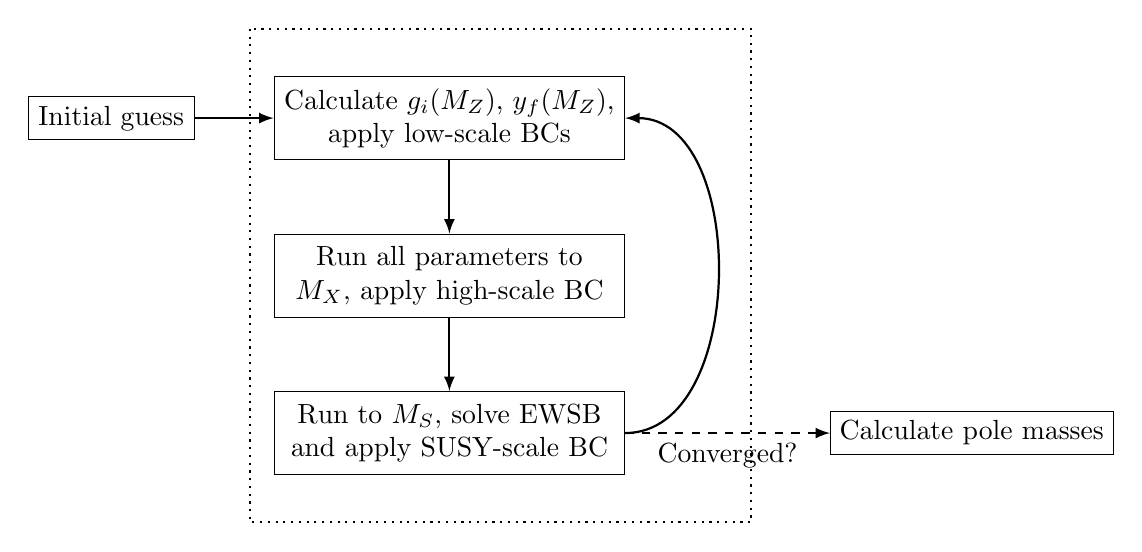
\begin{tikzpicture}[node distance = 2cm, auto]
        \tikzstyle{block} = [rectangle, draw, text width=12em,
                             text centered, minimum height=3em]
        \tikzstyle{arrow} = [draw, -latex, thick]
        \node[block] (MZ)
          {Calculate $g_i(M_Z)$, $y_f(M_Z)$, apply low-scale BCs};
        \node[block, below of=MZ] (MX)
          {Run all parameters to $M_X$, apply high-scale BC};
        \path[arrow] (MZ) -- node {} (MX);
        \node[block, below of=MX] (MS)
          {Run to $M_S$, solve EWSB and apply SUSY-scale BC};
        \path[arrow] (MX) -- node {} (MS);
        \path[-latex, thick] (MS.east) edge[bend right=90]
                             node[right] {} (MZ.east);
        \draw[thick,dotted] ($(MZ.north west)+(-0.3,0.6)$) rectangle
                            ($(MS.south east)+(1.6,-0.6)$);
        \node[rectangle, draw, minimum width=6em, text centered,
              left = 1cm of MZ] (guess) {Initial guess};
        \path[arrow] (guess) --node {} (MZ);
        \node[rectangle, draw, minimum width=10em, text centered,
              right = 2.6cm of MS] (pole) {Calculate pole masses};
        \path[arrow,dashed,below] (MS) --node {Converged?} (pole);
      \end{tikzpicture}
    \end{figure}
\end{frame}

\begin{frame}
  \frametitle{Semi-analytic Algorithm}
  \begin{figure}
    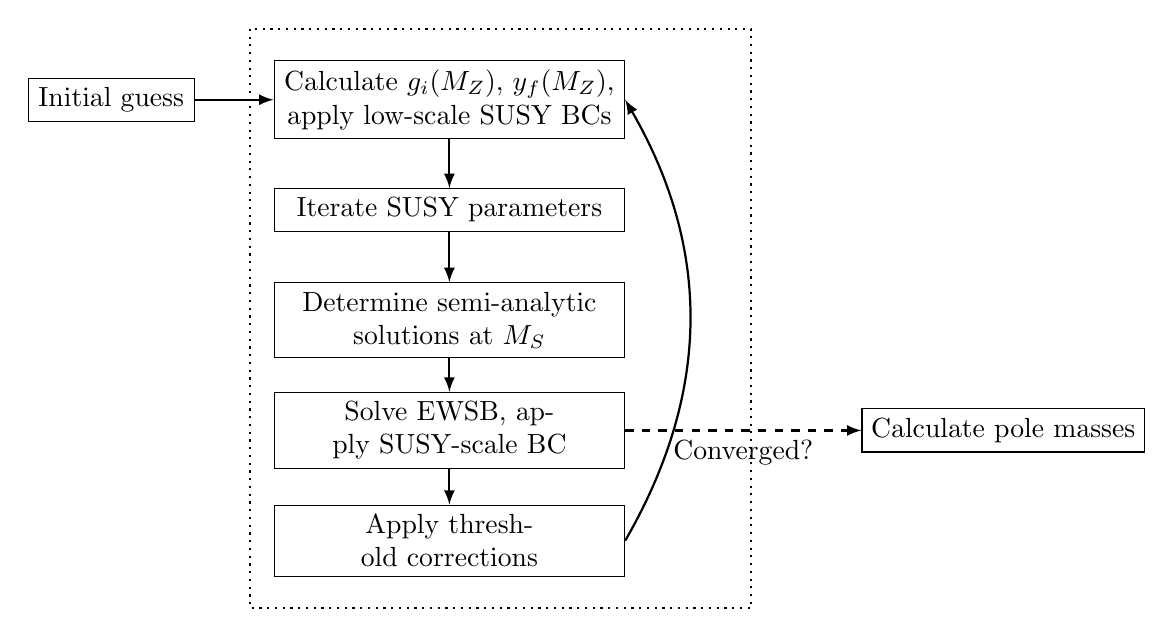
\begin{tikzpicture}[node distance = 1.4cm, auto]
      \tikzstyle{block} = [rectangle, draw, text width=12em,
                           text centered, minimum height=1.5em]
      \tikzstyle{arrow} = [draw, -latex, thick]
      \node[block] (MZ)
        {Calculate $g_i(M_Z)$, $y_f(M_Z)$, apply low-scale SUSY BCs};
      \node[block, below of=MZ] (susy) {Iterate SUSY parameters};
      \path[arrow] (MZ) --node {} (susy);
      \node[block, below of=susy] (coeffs)
        {Determine semi-analytic solutions at $M_S$};
      \path[arrow] (susy) --node {} (coeffs);
      \node[block, below of=coeffs] (MS) {Solve EWSB, apply SUSY-scale BC};
      \path[arrow] (coeffs) --node {} (MS);
      \node[block, below of=MS] (thresh) {Apply threshold corrections};
      \path[arrow] (MS) --node {} (thresh);
      \draw[thick,dotted] ($(MZ.north west)+(-0.3,0.4)$) rectangle
                          ($(thresh.south east)+(1.6,-0.4)$);
      \node[rectangle, draw, minimum width=6em, text centered,
            left = 1cm of MZ] (guess) {Initial guess};
      \path[arrow] (guess) --node {} (MZ);
      \path[-latex, thick] (thresh.east) edge[bend right=30]
                           node[right] {} (MZ.east);
      \node[rectangle, draw, minimum width=10em, text centered,
            right = 3cm of MS] (pole) {Calculate pole masses};
      \path[arrow,dashed,below] (MS) --node {Converged?} (pole);
    \end{tikzpicture}
  \end{figure}
\end{frame}

\begin{frame}
  \frametitle{CP-even Higgs Mass in the CSE$_6$SSM}
  \begin{columns}[t]
    \begin{column}{0.4\textwidth}
      \vspace{-20pt}
      \begin{figure}
        \hspace*{-15pt}
        \includegraphics[width=7.5cm]{cse6ssm_pos_mueff_1TeV_MSu6_MGlu_Mhh1}
      \end{figure}
      \vspace{-20pt}
      \begin{center}
        \tiny [\href{https://arxiv.org/abs/1610.03374}{arXiv:1610.03374}]
      \end{center}
      \begin{center}
        $m_{h_1} \lesssim 130$ GeV\\(i.e. bounded from above, as usual)
      \end{center}
    \end{column}
    \begin{column}{0.6\textwidth}
      \vspace{-20pt}
      \begin{itemize}
        \vfill
      \item {\color{red} Split spectrum $\Rightarrow$ large logarithms
        contribute}
          \vfill
        \item Exotic contributions small, mainly $\tilde{t}$'s
          \vfill
        \item Use EFT calculation of $m_{h_1}$
          (\href{http://users.ictp.it/susyhd/}{SUSYHD})
          \begin{itemize}
          \item cross-checked with prototype
            \href{http://flexiblesusy.hepforge.org/}{FlexibleEFTHiggs}
          \end{itemize}
          \vfill
      \end{itemize}
      \vspace{-10pt}
      \begin{figure}
        \includegraphics[width=7.5cm]{cmssm_pos_mueff_1TeV_MSu6_MGlu_Mhh1}
      \end{figure}
    \end{column}
  \end{columns}
\end{frame}

\begin{frame}
  \frametitle{$A$-funnel in the CSE$_6$SSM}
  \begin{columns}[t]
    \begin{column}{0.5\textwidth}
      \begin{itemize} \itemsep1.5em
        \vfill
      \item Solutions at lower $M_{1/2}$ due to
        $m_{A_1} \sim 2 m_{\tilde{\chi}_1^0}$
        \vfill
      \item CMSSM: $A$-funnel requires $\tan\beta \gtrsim 40$
        \vfill
      \item CSE$_6$SSM: tune $A_0$ for given $\tan\beta$, $M_{1/2}$ to that
        $m_{A_1} \rightarrow 0$, keeping $m_{\tilde{\chi}_1^0} \sim$ fixed
        \vfill
      \item Lightest state $A_1$ mixture of singlets for $s \gg M_S \gg v$
        ($\tan\delta \approx \frac{s_1 s_2}{\varphi \sqrt{s_1^2 + s_2^2}}$):
        \vfill
      \end{itemize}
    \end{column}
    \begin{column}{0.5\textwidth}
      \vspace{-55pt}
      \begin{figure}
        \includegraphics[width=8cm]{cmssm_a_funnel}
      \end{figure}
    \end{column}
  \end{columns}
  \vspace{10pt}
  \begin{equation*}
    m_{A_1}^2 \approx \cos^2\delta \left ( -2 B\mu
    - 3 \frac{\kappa A_\kappa}{\sqrt{2}} \varphi
    - \sqrt{2} \xi \frac{\Lambda}{\varphi} + \frac{9}{2}
    \sigma \kappa s_1 s_2 + 2\sqrt{2} \frac{\sigma \mu s_1 s_2}{\varphi}
    + \frac{\sigma s_1 s_2 \Lambda}{\varphi^2} \right )
  \end{equation*}
\end{frame}

\end{document}
